\documentclass[windows,csize4]{BHCexam}
%\documentclass[windows,csize4,answers]{BHCexam}

\usepackage{multicol} % 分栏
\pagestyle{fancy}
\fancyfoot[C]{\kaishu \small 第 \thepage 页 共 \pageref{lastpage} 页}
%\fancyhead[L]{\includegraphics[width=2cm]{qrcode.png}}
\title{因式分解 - 双十字相乘,主元法}
%\subtitle{数学文科试卷}
%\notice{满分150分, 120分钟完成, \\	允许使用计算器,答案一律写在答题纸上.}
%\author{Gavin Chen}
%\date{\today}
\usepackage{enumerate} % 编号

\begin{document}

\maketitle

\begin{groups}
    \group{双十字相乘概念}{}
        假设多项式
        \begin{equation}
        ax^2+bxy+cy^2+dx+ey+f \label{eq:factorization1} 
        \end{equation}
        可以因式分解为
        \begin{equation}
            (mx+py+j)(nx+qy+k) \label{eq:factorization2}
        \end{equation}
        将\ref{eq:factorization2}展开可以得到
        \begin{equation}
            mnx^2+(mq+np)xy+pqy^2+(mk+nj)x+(pk+qj)y+kj \label{eq:factorization3}
        \end{equation}

        根据多项式相等的原理,由\ref{eq:factorization1}和\ref{eq:factorization3}可以得到:
        \begin{equation}
            \begin{cases}
                mn=a \\
                mq+np=b \\
                pq=c  \\
                mk+nj=d \\
                pk+qj=e \\ 
                kj=f
            \end{cases}
            \label{eq:factorization4}
        \end{equation}
        所以可以得到双十字相乘
        \begin{figure}[htb]
            \centering
            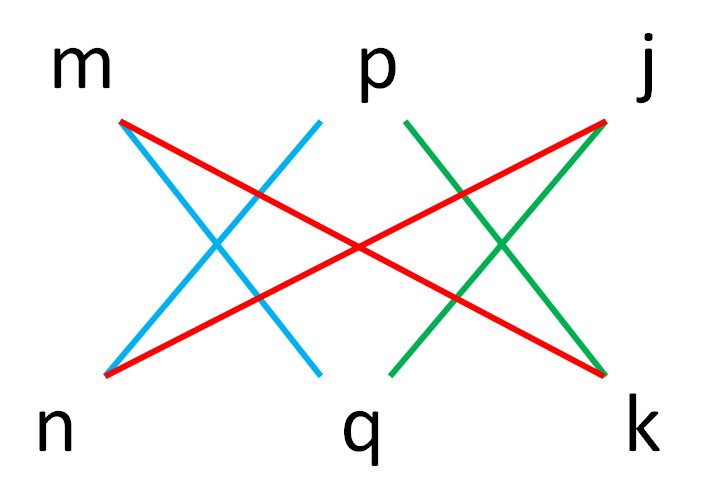
\includegraphics [scale=0.5,trim=0 0 0 0]{./image/U2_Factorization_1.png}
            \caption{双十字相乘示意图}
            \label{fig:factorization}
        \end{figure}
\end{groups}

\begin{groups}

    \group{双十字相乘例题}{}
    \begin{questions}[]
        \question[5]$x^2+3xy+2y^2+2x+2y+1$
        \begin{solution}{0.5cm}
            \methodonly $(x+y+1)(x+2y+1)$
        \end{solution}
        \vspace{3.5cm}

        \question[5]$x^2+2xy+y^2-3x-3y-40$
        \begin{solution}{0.5cm}
            \methodonly $(x+y-8)(x+y+5)$
        \end{solution}
        \vspace{3.5cm}





    \end{questions}

\end{groups}
\label{lastpage}
\end{document}